% !TEX TS-program = pdflatex
% !TEX encoding = UTF-8 Unicode

% This is a simple template for a LaTeX document using the "article" class.
% See "book", "report", "letter" for other types of document.

\documentclass[11pt]{article} % use larger type; default would be 10pt

\usepackage[utf8]{inputenc} % set input encoding (not needed with XeLaTeX)

%%% Examples of Article customizations
% These packages are optional, depending whether you want the features they provide.
% See the LaTeX Companion or other references for full information.

%%% PAGE DIMENSIONS
\usepackage{geometry} % to change the page dimensions
\geometry{a4paper} % or letterpaper (US) or a5paper or....
% \geometry{margin=2in} % for example, change the margins to 2 inches all round
% \geometry{landscape} % set up the page for landscape
%   read geometry.pdf for detailed page layout information

\usepackage{graphicx} % support the \includegraphics command and options

% \usepackage[parfill]{parskip} % Activate to begin paragraphs with an empty line rather than an indent

%%% PACKAGES
\usepackage{booktabs} % for much better looking tables
\usepackage{array} % for better arrays (eg matrices) in maths
\usepackage{paralist} % very flexible & customisable lists (eg. enumerate/itemize, etc.)
\usepackage{verbatim} % adds environment for commenting out blocks of text & for better verbatim
\usepackage{subfig} % make it possible to include more than one captioned figure/table in a single float
% These packages are all incorporated in the memoir class to one degree or another...

%%% HEADERS & FOOTERS
\usepackage{fancyhdr} % This should be set AFTER setting up the page geometry
\pagestyle{fancy} % options: empty , plain , fancy
\renewcommand{\headrulewidth}{0pt} % customise the layout...
\lhead{}\chead{}\rhead{}
\lfoot{}\cfoot{\thepage}\rfoot{}

%%% SECTION TITLE APPEARANCE
\usepackage{sectsty}
\allsectionsfont{\sffamily\mdseries\upshape} % (See the fntguide.pdf for font help)
% (This matches ConTeXt defaults)

%%% ToC (table of contents) APPEARANCE
\usepackage[nottoc,notlof,notlot]{tocbibind} % Put the bibliography in the ToC
\usepackage[titles,subfigure]{tocloft} % Alter the style of the Table of Contents
\renewcommand{\cftsecfont}{\rmfamily\mdseries\upshape}
\renewcommand{\cftsecpagefont}{\rmfamily\mdseries\upshape} % No bold!

%Tikz INI
	
\usepackage{tikz}
\usetikzlibrary{arrows}

%LSTListings
\usepackage{listings}
\usepackage{tabularx}
%algorithm
\usepackage{algorithm}
\usepackage{algorithmic}
%%% END Article customizations

%%% The "real" document content comes below...

\title{KI sheet}
\author{Benjamin Binder (1226121)}
%\date{} % Activate to display a given date or no date (if empty),
         % otherwise the current date is printed 

\begin{document}
\maketitle

\section{Exercise 1}

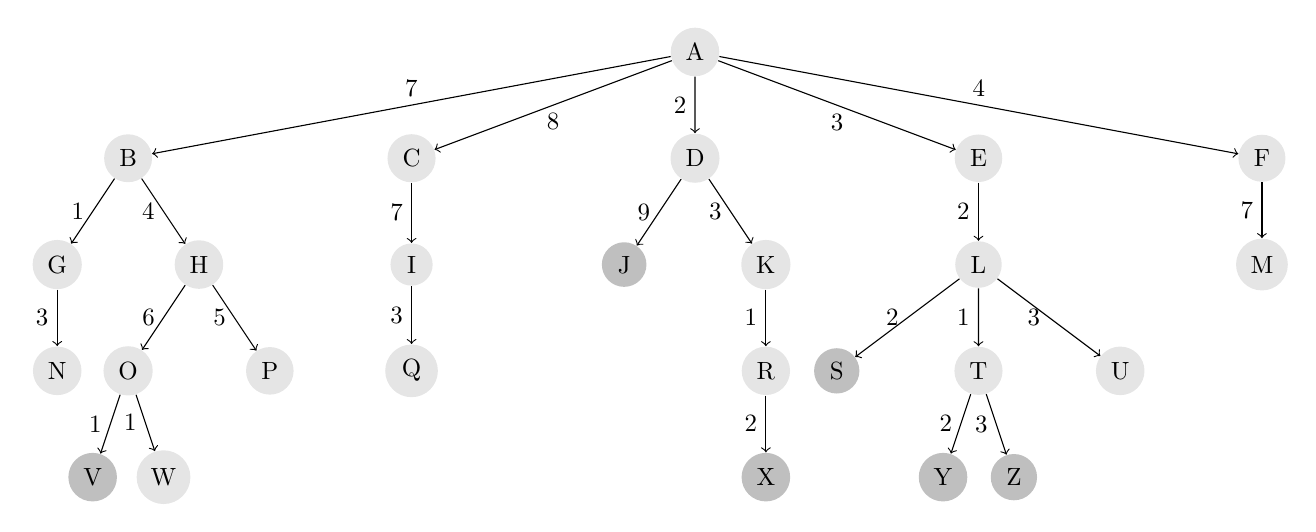
\begin{tikzpicture}[scale=.9, transform shape, edge from parent/.style={->, draw}, level 1/.style={sibling distance=40mm}, level 2/.style={sibling distance=20mm}, level 4/.style={sibling distance=10mm}]
	\tikzstyle{node} = [circle, fill=gray!20]
	\tikzstyle{targetNode} = [circle, fill=gray!50]
	\node[node] {A}
   		 child
   		 { 
   		 	node[node] {B} 
           		child
           		{
           			node[node] {G}   
            			child
            			{ 
            				node[node]{N} edge from parent node[left] {$3$}
				} edge from parent node[left]{$1$}
            		}
			child
           		{
           			node[node] {H}   
            			child
            			{ 
            				node[node]{O}
            				child
            				{
            					node[targetNode]{V} edge from parent node[left]{$1$}
            				}
            				child
            				{
            					node[node]{W}edge from parent node[left]{$1$}
            				} edge from parent node[left]{$6$}
				} 
				child
				{
					node[node]{P} edge from parent node[left]{$5$}
				}edge from parent node[left]{$4$}
            		}edge from parent node[above]{$7$}
    		}
            	child
            	{	
            		node[node]{C}
            		child
            		{
            			node[node]{I}
            			child
            			{
            				node[node]{Q}edge from parent node[left]{$3$}
            			}edge from parent node[left]{$7$}
            		}edge from parent node[below]{$8$}
            	}
           	child
            	{
            		node[node]{D}
            		child
            		{
            			node[targetNode]{J} edge from parent node[left]{$9$}
            		}
            		child
            		{
            			node[node]{K}
            			child
            			{
            				node[node]{R}
            				child
            				{
            					node[targetNode]{X} edge from parent node[left]{$2$}
            				} edge from parent node[left]{$1$}
            			} edge from parent node[left]{$3$}
            		} edge from parent node[left]{$2$}
            	}
            	child
            	{
            		node[node]{E}
            		child
            		{
            			node[node]{L}
            			child
            			{
            				node[targetNode]{S} edge from parent node[left]{$2$}
            			}
            			child
            			{
            				node[node]{T}
            				child
            				{
            					node[targetNode]{Y} edge from parent node[left]{$2$}
            				}
            				child
            				{
            					node[targetNode]{Z} edge from parent node[left]{$3$}
            				} edge from parent node[left]{$1$}
            			}
            			child
            			{
            				node[node]{U} edge from parent node[left]{$3$}
            			} edge from parent node[left]{$2$}
            		} edge from parent node[below]{$3$}
            	}
            	child
            	{
            		node[node] {F}
            		child
            		{
            			node[node]{M} edge from parent node[left]{$7$}
            		} edge from parent node[above]{$4$}
            	}
	;
\end{tikzpicture}


Determine for the following search strategies the order in which the nodes are expanded and the
corresponding goal node. In case you can expand several nodes and the search strategy does not
specify the order, choose the nodes in alphabetic sequence. In addition, compute for each search
strategy the set of nodes that is actually kept in memory when the goal node is found (node A has
depth zero).




\subsection{Breadth First Search}

Uses a FIFO Queue to queue the Nodes visited. Also there is a explored List to avoid circular searching.


\begin{algorithm}
\caption{breadth-first-search }
\begin{algorithmic} 

\STATE $node \leftarrow $a node with STATE=problem.INITIAL-STATE
\STATE PATH-COST = 0
\IF{ problem.GOAL-TEST(node.STATE)}
\STATE
\RETURN node
\ENDIF
\STATE $frontier \leftarrow $a FIFO queue with node as the only element
\STATE $explored \leftarrow $an empty set
\LOOP
	\IF {EMPTY?(frontier)}
		\STATE 
		\RETURN failure
	\ENDIF
	\STATE $node \leftarrow $POP(frontier) /*chooses the shallowest node in frontier */
	\STATE node.STATE = explored
	\FOR{\textbf{each} action in problem.ACTIONS(node.STATE) }
	\STATE $child \leftarrow $CHILD-NODE(problem, node, action)
	\IF {child.STATE is not in explored or frontier}
		\IF {problem.GOAL-TEST(child.STATE)}
			\STATE
			\RETURN child
		\ENDIF
		\STATE $frontier \leftarrow $INSERT(child, frontier)
	\ENDIF
	\ENDFOR
\ENDLOOP


\end{algorithmic}
\end{algorithm}
\begin{tabularx}{\textwidth}{|r|c|X|X|}
\hline
node & frontier & explored  \\
\hline
0&A&0\\
\hline
A&B, C, D, E, F&0\\
\hline
B&C, D, E, F, G, H&A\\
\hline
C& D, E, F, G, H, I&A, B\\
\hline
...& ...&A, B, ...\\
\hline
J&K, L, M, N, O , P, Q&A, B, C, D, E, F, G, H, I\\
\hline
\end{tabularx}

\begin{tabularx}{\textwidth}{|r|c|X|X|}
\hline
node & frontier & explored  \\
\hline
J&K, L, M, N, O , P, Q&A, B, C, D, E, F, G, H, I\\
\hline
...& ...&A, B, ...\\
\hline
S&T, U, V, W, X&A, B, C, D, E, F, G, H, I, J, K ,L ,M, N, O, P, Q, R\\
\hline
\end{tabularx}

\begin{tabularx}{\textwidth}{|r|c|X|X|}
\hline
node & frontier & explored  \\
\hline
S&T, U, V, W, X&A, B, C, D, E, F, G, H, I, J, K ,L ,M, N, O, P, Q, R\\
\hline
...& ...&A, B, ...\\
\hline
V&W, X, Y, Z&A, B, C, D, E, F, G, H, I, J, K ,L ,M, N, O, P, Q, R, S, T, U, V\\
\hline
\end{tabularx}

\begin{tabularx}{\textwidth}{|r|c|X|X|}
\hline
node & frontier & explored  \\
\hline
V&W, X, Y, Z&A, B, C, D, E, F, G, H, I, J, K ,L ,M, N, O, P, Q, R, S, T, U, V\\
\hline
...& ...&A, B, ...\\
\hline
X&Y, Z&A, B, C, D, E, F, G, H, I, J, K ,L ,M, N, O, P, Q, R, S, T, U, V, W\\
\hline
\end{tabularx}

\begin{tabularx}{\textwidth}{|r|c|X|X|}
\hline
node & frontier & explored  \\
\hline
X&Y, Z&A, B, C, D, E, F, G, H, I, J, K ,L ,M, N, O, P, Q, R, S, T, U, V, W\\
\hline
...& ...&A, B, ...\\
\hline
Y&Z&A, B, C, D, E, F, G, H, I, J, K ,L ,M, N, O, P, Q, R, S, T, U, V, W,X\\
\hline
\end{tabularx}

\begin{tabularx}{\textwidth}{|r|c|X|X|}
\hline
node & frontier & explored  \\
\hline
Y&Z&A, B, C, D, E, F, G, H, I, J, K ,L ,M, N, O, P, Q, R, S, T, U, V, W,X\\
\hline
...& ...&A, B, ...\\
\hline
Z&empty&A, B, C, D, E, F, G, H, I, J, K ,L ,M, N, O, P, Q, R, S, T, U, V, W, X, Y\\
\hline
\end{tabularx}


\subsection{Uniform Cost Search}




\end{document}
